\chapter{Performance Analysis}
 %This section  .... table \ref{table:2} \cite{r2}
\section{Fuzzification}
\subsection{Fuzzification Method:}
\textbf{Fuzzy logic} is a form of 
\begin{itemize}
    \item Fuzzification Unit
    \item Knowledge Based Rules
    \item Decision or Controller Unit
    \item Defuzzification Unit
\end{itemize}

%% to write equation; table and figure you have to start with \begin

\begin{equation}
    y=\cos(x)+\sin(x) +\beta
\end{equation}

where $y$ is the output of the system and $x$ is the input of the system.

\begin{figure}[ht!] %H--- must here; h-- here, t--top, b--bottom
    \centering
    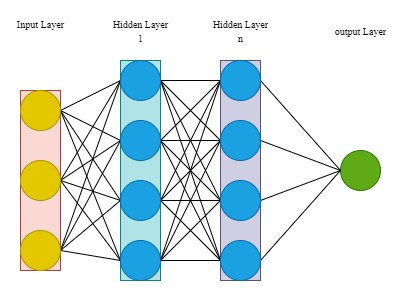
\includegraphics[scale=0.5]{Chap5/cnn1.jpg}
    \caption{CNN architecture}
    \label{fig:CNN}
\end{figure}


Figure \ref{fig:CNN} shows a CNN architecture. 


\begin{table}[]
    \centering
    \caption{Deep learning Algorithms \cite{mondal_automatic_2017}}
    \begin{tabular}{cp{2in}} %c--center, l--left, r--right; p-- width
      \hline %horizontal line
      \textbf{Name of Algorithm}   & \textbf{Description}  \\ \hline
        CNN & It includes input, hidden and output layers .\\ \hline
        RNN & It is useful for time series data. It takes output and fed into input \\ \hline
    \end{tabular}
        \label{tab:DL}
\end{table}

Table  \ref{tab:DL}     shows deep learning algorithm \cite{wiki_2016}.


